%!TEX root = ../../super_main.tex
\section{Vision}
\label{sec:vision}

We would like to develop a platform that allows for dynamic collection of data for reality mining. Different area of reality mining require different types of labeled training data. For this reason the platform should allow for configurable campaigns of data collection. A customer should be able to to configure what type of data he wants in the set of training data and how the entries should be labeled. The vision for the platform is that people that are in needed of context aware training data can use our platform instead of developing and distributing their own specialized applications to gather these type of data. We imagine that our platform will handle all technical details in regard of gathering the training data, and the only task that is left for the customers of this platform is to motivate participants, which they would have to do in any case.

\todo[inline]{Find a place for this sentence}

% Vi har ikke nogen udefrakommende kunne, vi vil håndtere dette med et essence vision
This project aims to be innovative and does not have an external customer whom can define and verify requirements. 
\\\\
A software development methodology that aims to support high value software solutions is Essence \parencite{essence_book}. Essence mentions having a vision as a great way to start a project. Essence mentions that having different representations of a vision can help elicit objects, events, and qualities to persue. Four different representation types are suggested, namely: Icon, Prototype, Metaphor, Proposition. We have chosen to attempt to represent the existing condition, i.e. the problem area as we understood it at the time, as Icons, Metaphors, and Propositions. We found the prototype representation too costly in terms of development time. 

\subsection{Start Configuration}
\label{sub:start_configuration}

\todo[inline]{Consider the term subject vs user, in terms of medical subject makes great sense but can we use that term instead of user?}
As described in \secref{sub:essence_start_configuration}, the start configuration is the basis foundation on which the entire system can mature. In this section we describe existing solutions, potentially interesting and useful infrastructure, and high level design patterns, which could contribute with ideas to the development of our system.

\subsubsection{Existing Solutions}

Some solutions that uses data gathering in the world of mental health have been investigated. It seems that a lot of software have been designed to improve mental health using mobile sensor data gathering. We will discuss two solutions that both monitor subjects using smartphone sensors and have these subjects fill out surveys. 
\\\\
There exists a concept called Ecological Momentary Assessment (EMA) \parencite{shiffman2008ecological} in mental health care, which is a way of making assessments of patients in the ecosystem where they normally exist. In traditional medical practice the patient is acquainted with a doctor, where long term treatment is periodical appointments with a doctor. This particular pattern has disadvantages in psychological treatments where the treatment does not happen in the environment where the patient lives, but it happens in a doctors or psychiatrist office. EMA is a way of gathering information from patient and possibly providing some sort of treatment or intervention in real-time. This type of system works particularly well using mobile technologies.
\\\\
Ilumivu\footnote{http://ilumivu.com/solutions/ecological-momentary-assessment-app/} have developed a Mobile EMA (mEMA) application. This application provides researchers and companies with a platform for real-time data gathering from test subjects going about their daily lives. The functionality in the purchasable core package of mEMA includes questionnaires and creation of these. It is also possible for the customers to add certain opt-ins that can provide more context for the answers of the questionnaires, such as mobile sensors, wearable sensors, and in-home sensors. The system is centered around the patient, and is generally meant for research purposes.
\\\\
% AndWellness
AndWellness \parencite{hicks2010andwellness}, is another sensor monitoring/questionnaire focused system for Android phones. AndWellness have some interesting points on architecture and principles to do this type of monitoring. This system has a concept of a campaign which is the definition of studies, meaning it is the configuration of how sensor data is gathered and surveys are filled on the subjects smartphones. These configurations include how sensors should be monitored in terms of frequency and duration. It is also possible to configure how subjects are notified. AndWellness allows configuration of different triggers for questionnaires. These triggers can be set to be both temporal but also sensor activity based, meaning that both time and the activity and movement of the user can trigger sensor monitoring and notifications with surveys. This means that the customers using AndWellnes is able to customize their study in great detail, which is preferable as the purpose of the gathered data may vary. Lastly an idea to note is that this system has a concept of expiring surveys, meaning that the customer can configure for how long the subject may prolong a survey with a time window where the survey exists. These time windows allows customers to disallow meta cognition, the process of reflecting about ones thoughts. Some mental health studies does not want meta cognitions, i.e. no reflection after some activity, while other studies include meta cognitions as an important factor. 
\\\\
The AndWellness system allows for full transparency, meaning that subjects have full access to the data they are gathering for the customers, to increase trustworthiness. Lastly AndWellness does not support raw sensor output logging, they derive some soft sensors which they call Location- and Activity trace sensors. This is a potential flaw, because the data used to derive output cannot be converted back to raw sensor output and a mental health study might need data which is not included in the outputs of these predefined soft sensors.
\\\\
mEMA and AndWellness both monitor and report sensor readings in real time, meaning that they are highly connectivity dependent. It is not clear what these systems do in cases where there is no network access, but they stream the data directly to a server in almost real time when the phone is connected to a network. This type of network communication is counter intuitive with general practices on battery and network management. Furthermore these systems do not yet include a larger ecosystem of devices. For instance, these systems do not consider wearable technologies such as smartwatches and smartbands. This excludes some potential sensor information which is usually not present in smartphones.

% + Principle of campaign. %
% + Sensor monitoring have configurable resolutions (our terms: measurement frequency, sample duration, sample frequency).
% + Have different triggers, temporal, contextual (sensor). 
% + Triggers can both be camgaign-wise and participant specific.
% + Prompts for surveys.
% + Surveys expire, configured by admins of campaign (answering window).
% + Users have full transparency of the data gathered
% - Pure realtime, battery drain, very network dependent.
% - Pure smartphone, no wearable technology.
% - Only two derived (software sensors), Location and Activity tracing.
%     - No raw sensor output

\subsubsection{Data Collection Applications}

\todo[inline]{The two previously mentioned apps also collect data?}

% Purple Robot
Purple Robot\footnote{https://tech.cbits.northwestern.edu/purple-robot/} is an Android application originally developed to allow for easier or better integration for the PhoneGap and Apache Cordova applications with native functionality on the Android platform. The application allows other non-native applications to trigger status-bar notifications, application widgets, and full native dialogs. The application also allows other applications to access all the sensors on a device with an uniform interface. 
The communication for triggering and reading of the sensors is done using a locally running HTTP server that the Purple Robot application runs. This means that the Purple Robot application actually does not provide a lot of functionality for a user on its own, but allows other applications to have easy access to the integrated native functionality.
% This framework could be used to create what we are striving for?
This framework could be used to create access to native functionality, i.e. the sensors of an Android device, without having to build and maintain an Android application. Users could be asked to download and install Purple Robot instead. The framework supports delayed and encrypted uploads of collected data. 
\\\\
Like Purple Robot, Sensor Data is an iPhone application for gathering unlabeled data. The application can gather data from all the sensors that are available in iPhone devices, which is then made available through a web API. It is possible to store the sensor data in two different ways when using Sensor Data: Capture Mode and Streaming Mode. When using Capture Mode the data is stored directly into the flash memory of the iPhone, while using Streaming Mode will transfer the data to another computer. The data is recorded and stored as comma separated values for easy integration into data analysis software.
\\\\
%Trust in third part
It might already be challenge for us to gain the trust of users. We are handling sensitive information about their everyday activities and life. 
Installing a third part application to handle this information could become a potential trust issue. We have installed the Purple Robot application on our devices and found the graphical user interface in the application to be unstable with seemingly random breakdowns. We have found this application and concept interesting, but we have found the application too unstable to be practical.   

\todo{The data sensor collection costs money!}
\subsubsection{Design Patterns and General Strategies}

Sloppy handling of network communication is seen as a common source of battery drain \parencite{android_network_scheduling} in the Android development community. Gathering training data with the purpose of training an AI model does not require the training data to be delivered in real time unless the model itself is actually required to be trained and completed within a given temporal frame. 
\\\\
Several different tactics and techniques can be utilized in order to minimize battery drain. A common method to reduce network communication is to compress the data being sent \parencite{har_wearables}\parencite{android_network_scheduling}. This reduces the amount of data that has to be transferred, i.e. the amount of packets, and the awake-time of the network module. Another possibility is to communicate in bulks, which means that instead of sending many small packages with breaks in between, these can be collected into bigger packets. This will reduce the overhead of activating the module. The bulk transfer solution requires the data to be aggregated over time, which requires some sort of intermediate storage. This can be achieved by storing the data in memory for small data packets or persistently on a device for larger packets. Storing the data persistently on the device will also remove the risk of losing the data due to device crashes, and the data therefore becomes less volatile. Another side-effect of storing data, either persistently or in memory, is the possibility collecting data when there is no available connection or only a connection with a high power consumption, e.g. cellular network, and then sending it when a desired connection becomes available. 
\\\\
Other typical techniques for reducing power consumption include \parencite{android_network_scheduling}:

\begin{itemize}
    \item Pre-fetch network data
    \item Network scheduling services (use the network when other uses it).
    \begin{itemize}
        \item Bundle outgoing data (cache outgoing data)
    \end{itemize}
    \item Reduce number of connections
\end{itemize}

The idea of aggregating and minimizing network communication in a sensor network to save power is not a novel one \parencite{korteweg2007data} \parencite{mhatre2004design}, but they are not included features in the sensor data collecting applications described in \secref{sub:start_configuration}. A battery consumption aware application which collects data, but does not synchronize it with a server in real time, could offer substantial battery consumption improvements to existing solutions. 

\subsection{Vision Scenarios}
\label{sub:vision_scenarios}

% Essence suggests finding two fundamentally opposing questions that properly represent different directions the project could take. This allows for a clearer insight in the benefits of progressing in either way. The overall goal of this exercise is to explore the design space and to learn more about what we want to create, and eventually end up with a vision for the project. The Essence book has an example project called Psyche where several different opposing questions were found, such as Intervention vs Observation and Citizen Oriented vs Caretaker Oriented. Essence furthermore suggests the four previously mentioned representations for each direction of the two questions, which is typically represented by using the four quadrants in a graph representation. One can start by finding several opposing questions, and then selecting the two most central ones. 
Essence, as mentioned in \secref{sub:essence_vision_scenarios}, a suggests to utilize vision scenarios. We have come up with a list of opposing directions of development, which can be used to explore the different quadrants of a graph with two of the opposites as its axes. The purpose of this is to detail different directions the project could take and thereby learn more about the problem and possibly learn more about how it can be sovled. 

\begin{itemize}[itemsep=0.1em]
	\item Disruptive/Non-disruptive - Should the system be based on passively collected sensor data or interactively prompt with questionnaires? % 1
	\item On demand/Continuous - Should the system be activated by users or run continuously in the background? % 2
	\item Easy-of-use/Customizable - Should we require that customers must customize campaigns or should it be ``one data collection configuration fits all''? % 3
	\item Assigned/Opt-in - Should campaigns be assigned automatically to users using a user profile or should users actively choose campaigns? % 4
	\item Personal/Anonymous - Should the system require personal information about users or not? % 5
\end{itemize}

We have chosen to use the Ease-of-use/Customizable and Assigned/Opt-in orientation questions as axes. 
\\\\
% 1
We found it difficult to imagine the usefulness of a system that exclusively collects sensor data for classification problems. This means that at least some data not based on sensor should be collected. The degree of disruptiveness could then perhaps be regulated by the campaign configuration. 
% 2
The system could allow users to turn the system on/off easily but we think that having the system running continuously once activated would increase the probability of completing campaigns. Actual data collection would also depend on whether there is one or more active campaigns on the user's device.
% 5
We found that some demographic information would be necessary for both the scenario where users are assigned to campaigns and where they opt-in. Customers would likely be interested in whether the collected data represents the wide population or the specific group they are targeting for their data collection project. The degree of personal information required for a given campaign could perhaps also be defined in a campaign configuration. 
\\\\
We have chosen to include Static/Customizable because we thought it would be interesting to explore different ways of allowing customers to configure what data they want and how they want it and because we think that both direction could add value. We have chosen Assigned/Opt-in because these directions would have a large impact on how a solution should be formed. We would have to store a lot of demographic data about participants, thereby possibly impacting privacy, if we want to assign and match campaigns. Both directions would impact how the interaction with participants should be designed and what the server side should do in different ways.




% 1: rå sensor data har begrænset anvendelsesmuligheder --> spørgeskema kan hjælpe med dette.
% 		brug for en eller anden grad af labels fra brugere. Behøver ikke komme fra spørgeskemaer

% 2: Skal bruger forstyrres "unødvendigt" eller selv aktivt starte appen op fx. hver dag eller skal den køre i baggrunden
% Fordel ved selv styring er at de kan regulere strøm forbrug og vælge hvilke dag de vil deltage. Ulempe ved at de vælger er at det kan være svært at generalisere over tid. 
% Begge dele kan påvirker bruger entusiasmen/involveringen

% 3: Skal det være nemt/hurtigt at lave campaigns

\subsection{Icon Representation}


\subsection{Metaphor Representation}


\subsection{Proposition Representation}


\begin{figure}[!htbp]
    \centering
    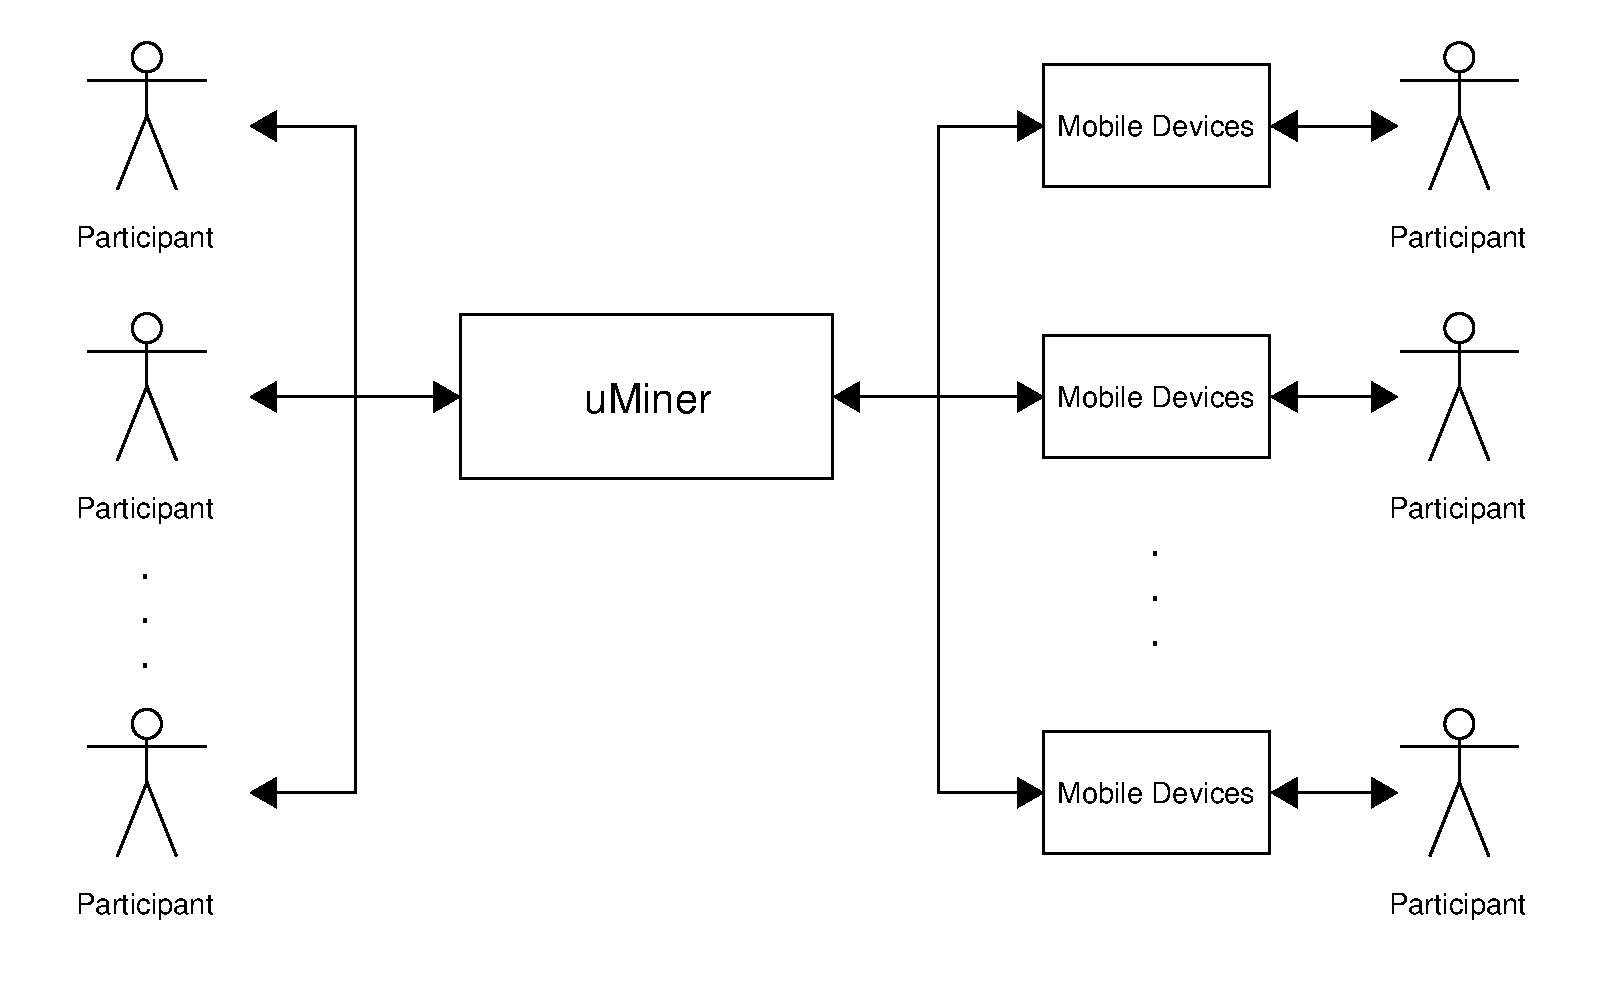
\includegraphics[width=\textwidth]{unsorted/system_vision}
    \caption{The system vision.}
    \label{fig:system_vision}
\end{figure}
\FloatBarrier
